\documentclass[]{book}
\usepackage{lmodern}
\usepackage{amssymb,amsmath}
\usepackage{ifxetex,ifluatex}
\usepackage{fixltx2e} % provides \textsubscript
\ifnum 0\ifxetex 1\fi\ifluatex 1\fi=0 % if pdftex
  \usepackage[T1]{fontenc}
  \usepackage[utf8]{inputenc}
\else % if luatex or xelatex
  \ifxetex
    \usepackage{mathspec}
  \else
    \usepackage{fontspec}
  \fi
  \defaultfontfeatures{Ligatures=TeX,Scale=MatchLowercase}
\fi
% use upquote if available, for straight quotes in verbatim environments
\IfFileExists{upquote.sty}{\usepackage{upquote}}{}
% use microtype if available
\IfFileExists{microtype.sty}{%
\usepackage{microtype}
\UseMicrotypeSet[protrusion]{basicmath} % disable protrusion for tt fonts
}{}
\usepackage[margin=1in]{geometry}
\usepackage{hyperref}
\hypersetup{unicode=true,
            pdftitle={ArborPro Documentation},
            pdfauthor={Tyler Littlefield},
            pdfborder={0 0 0},
            breaklinks=true}
\urlstyle{same}  % don't use monospace font for urls
\usepackage{natbib}
\bibliographystyle{apalike}
\usepackage{longtable,booktabs}
\usepackage{graphicx,grffile}
\makeatletter
\def\maxwidth{\ifdim\Gin@nat@width>\linewidth\linewidth\else\Gin@nat@width\fi}
\def\maxheight{\ifdim\Gin@nat@height>\textheight\textheight\else\Gin@nat@height\fi}
\makeatother
% Scale images if necessary, so that they will not overflow the page
% margins by default, and it is still possible to overwrite the defaults
% using explicit options in \includegraphics[width, height, ...]{}
\setkeys{Gin}{width=\maxwidth,height=\maxheight,keepaspectratio}
\IfFileExists{parskip.sty}{%
\usepackage{parskip}
}{% else
\setlength{\parindent}{0pt}
\setlength{\parskip}{6pt plus 2pt minus 1pt}
}
\setlength{\emergencystretch}{3em}  % prevent overfull lines
\providecommand{\tightlist}{%
  \setlength{\itemsep}{0pt}\setlength{\parskip}{0pt}}
\setcounter{secnumdepth}{5}
% Redefines (sub)paragraphs to behave more like sections
\ifx\paragraph\undefined\else
\let\oldparagraph\paragraph
\renewcommand{\paragraph}[1]{\oldparagraph{#1}\mbox{}}
\fi
\ifx\subparagraph\undefined\else
\let\oldsubparagraph\subparagraph
\renewcommand{\subparagraph}[1]{\oldsubparagraph{#1}\mbox{}}
\fi

%%% Use protect on footnotes to avoid problems with footnotes in titles
\let\rmarkdownfootnote\footnote%
\def\footnote{\protect\rmarkdownfootnote}

%%% Change title format to be more compact
\usepackage{titling}

% Create subtitle command for use in maketitle
\newcommand{\subtitle}[1]{
  \posttitle{
    \begin{center}\large#1\end{center}
    }
}

\setlength{\droptitle}{-2em}

  \title{ArborPro Documentation}
    \pretitle{\vspace{\droptitle}\centering\huge}
  \posttitle{\par}
    \author{Tyler Littlefield}
    \preauthor{\centering\large\emph}
  \postauthor{\par}
      \predate{\centering\large\emph}
  \postdate{\par}
    \date{Last updated: 2018-12-04}

\usepackage{booktabs}

\begin{document}
\maketitle

{
\setcounter{tocdepth}{1}
\tableofcontents
}
\hypertarget{welcome}{%
\chapter*{Welcome}\label{welcome}}
\addcontentsline{toc}{chapter}{Welcome}

Welcome to ArborPro! Here, you can find everything you need to know
about ArborPro software. If you are reading this, we assume you already
have ArborPro software and are ready to dive into the details. However,
if this isn't the case and you are simply interested in what the
software has to offer, please contact us
\href{http://arborprousa.com/\#contacthome}{here}.

\hypertarget{intro}{%
\chapter{Introduction}\label{intro}}

ArborPro assists forestry managers with managing their tree maintenance.
The software incorporates a mapping component allowing the user to view,
select, and locate trees or groups of trees. The dynamic link between
the mapping component and the database provides a unique and powerful
tool.

\hypertarget{system-requirements}{%
\section{System Requirements}\label{system-requirements}}

ArborPro has the following system requirements:

\begin{itemize}
\tightlist
\item
  Windows 2000/XP/Vista/8/10
\item
  512MB RAM or greater
\item
  130MB disk space
\item
  Additional disk space for mapping data

  \begin{itemize}
  \tightlist
  \item
    Note: This can be up to many gigabytes for high-resolution aerial
    photography.
  \end{itemize}
\end{itemize}

\hypertarget{tree-inventory-methodology}{%
\section{Tree Inventory Methodology}\label{tree-inventory-methodology}}

Trees are located in the field using a Global Positioning System (GPS)
receiver. The ground coordinates are recorded and used to determine
several site characteristics, such as nearest street, zone, adjacent
building, and so on. Additionally, a number of tree characteristics are
assessed and recorded, including the height, diameter, structure,
condition, and species of the tree.

\hypertarget{quick-references}{%
\chapter{Quick Reference}\label{quick-references}}

This chapter is the \emph{``too long, didn't read''} (TLDR) section of
the documentation. It's meant for users that want to know how to do
stuff without diving into the knitty gritty details of it all.
Additionally, you can skip to chapter \ref{applications} for further use
cases.

\hypertarget{recording-work}{%
\section{Recording Work}\label{recording-work}}

The most common task involves recording work done on trees. The workflow
changes depending on whether or not we are recording work for a single
tree or multiple trees.

\hypertarget{one-tree}{%
\subsection{One Tree}\label{one-tree}}

To record work done on a single tree:

\begin{enumerate}
\def\labelenumi{\arabic{enumi}.}
\tightlist
\item
  Open ArborPro.
\item
  Locate the tree that needs work done to it.

  \begin{itemize}
  \tightlist
  \item
    You have two options for locating the tree: Search by
    characteristics or by simply zooming into the area of interest.
  \end{itemize}
\item
  Click on the Identify (``i'') tool and click on the tree.
\item
  Select the Work History tab. The list on the left side shows all
  recorded work that has been completed for this tree.
\item
  Click on the new work record button.
\item
  Fill in all the information on the right, click the Save button, and
  press . There are three dates: Date refers to the current date,
  i.e.~the date entered. Scheduled is a scheduled date and Completed is
  the date the work was actually done. Click the triangle next to each
  date field to see a calendar. This new work history record has now
  been added to the tree. If any crews or work types need to be
  modified, use the Edit \textgreater{} Maintenance Options menu to add
  or edit these items.
\end{enumerate}

\hypertarget{multiple-trees}{%
\subsection{Multiple Trees}\label{multiple-trees}}

To record work done on multiple trees:

\begin{enumerate}
\def\labelenumi{\arabic{enumi}.}
\tightlist
\item
  Open ArborPro.
\item
  Locate the trees that require work. Simliar to the above, we have two
  options: Using the select tool or search by characteristics\footnote{The
    select tool can be used to draw a box on the map to highlight
    several trees, or click on individual trees one-by-one. See the
    tools chapter for more information on how the select tool works.}.
\item
  Click on the ``Inventory'' tab and click on the ``List''
  button\footnote{A list allows you to apply work done to many trees,
    without having to enter work history individually for each tree.
    This can be a substantial time saver if you perform work on many
    trees at a time.}.
\item
  The New List window appears. This allows you to save the selected
  trees to a list. Enter the work code, sub code, crew, notes, and date
  the work was completed. Click ``OK'' to apply that work to all trees
  in the list. If you need to specify different dates the work was done,
  do not fill in a completion date and go to Step 5.
\item
  To fill in individual dates for work done, click on the List in the
  left side. It will appear under the ``Open Lists'' since a completion
  date was not specified. Drag the scroll bar at the bottom all the way
  to the right to see the Date column. Click on an empty date box and
  enter the date, i.e. ``1/20/18''. Use the Down Arrow key on your
  keyboard to automatically fill in the same date on the next row. Click
  on the ``Save'' button to finish.
\end{enumerate}

\hypertarget{tools}{%
\chapter{Tools}\label{tools}}

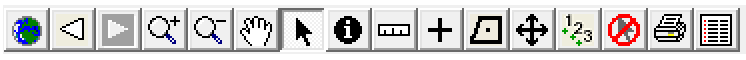
\includegraphics[width=10.36in]{images/toolbar}

We describe the tools ArborPro has to offer in this chapter. These tools
can be broken down into two categories: editing tools and navigation
tools. Editing tools allow users to modify the data and navigations
tools allow users to navigate the map and locate specific trees. Below
is a table that quickly summarises the tools:

\begin{tabular}{l|l}
\hline
Tool & Description\\
\hline
Full Extent & Zoom to the full map extent as defined by user\\
\hline
Zoom Previous & Zoom to previous map extent\\
\hline
Zoom Next & Zoom to the next map extent (assuming you've rolled back to a previous map extent)\\
\hline
Zoom In & Zoom in closer to the map image\\
\hline
Zoom Out & Zoom out farther away from map image\\
\hline
Pan & 'Pan and scan' the map by clicking and dragging the cursor\\
\hline
Select & Select trees by point and click, marquee selection, or polygon selection\\
\hline
Identify & Open the tree detail window of a tree\\
\hline
Measure & Measure distances\\
\hline
Add Tree & Add trees (points) to the map\\
\hline
Add Polygon & Draw polygons on the map\\
\hline
Move Point & Move trees (points) from one location to another\\
\hline
Site Numbering & Manually renumber tree sites\\
\hline
Clear Selection & Clear the current selected trees\\
\hline
Print Map & Print a map\\
\hline
List & Create a list\\
\hline
\end{tabular}

\hypertarget{tool-details}{%
\section{Tool Details}\label{tool-details}}

We've dedicated a section for each tool to go over in more detail.

\hypertarget{full-extent}{%
\subsection{Full Extent}\label{full-extent}}

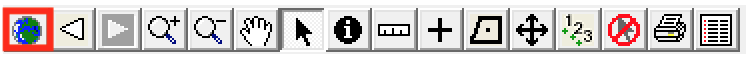
\includegraphics[width=10.36in]{images/toolbar-full-view}

When you open ArborPro it displays the \emph{default map extent}. Users
can modify that extent by going to \emph{Tools} then selecting \emph{Set
Default Map Extent}. The current map displayed will now be the default
map view everytime ArborPro is opened.

Often times, a tree inventory spans many miles and users will spend the
day working on multiple areas in the map. As a result, zooming out can
become time consuming. This is where the Full Extent tool becomes
useful, when users need to quickly zoom into an area, do some work and
then zoom back out to the full extent so that they can zoom into a
different area on the map. To zoom back to the full map view, simply
click the Full Extent tool.

\hypertarget{zoom-previous}{%
\subsection{Zoom Previous}\label{zoom-previous}}

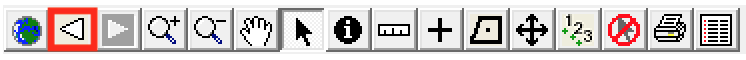
\includegraphics[width=10.36in]{images/toolbar-back-view}

This is another navigation tool that takes users to the previous map
extent. Occasionally, users might zoom into an area on accident in which
case, they want to go back to the previous map view. This is why the
Zoom Previous tool exists.

\hypertarget{zoom-next}{%
\subsection{Zoom Next}\label{zoom-next}}

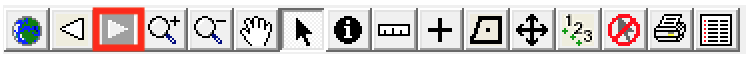
\includegraphics[width=10.36in]{images/toolbar-forward-view}

The Zoom Next tool is nearly identical to the Zoom Previous tool except
it sends the user to the next map extent.

\hypertarget{zoom-in}{%
\subsection{Zoom In}\label{zoom-in}}

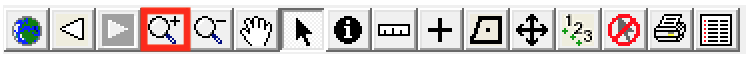
\includegraphics[width=10.36in]{images/toolbar-zoom-in}

One of the most important navigation tools, this allows users to zoom
into specific areas on the map. This can be done in two ways: point and
click or drawing a box to zoom into the area inside that box\footnote{The
  drawing a box method is often called \emph{Marquee Zoom}.}.

\hypertarget{zoom-out}{%
\subsection{Zoom Out}\label{zoom-out}}

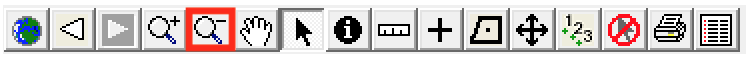
\includegraphics[width=10.36in]{images/toolbar-zoom-out}

Similar to the Zoom In tool with two exceptions: this zooms the user out
and you may only point and click to zoom out.

\hypertarget{pan}{%
\subsection{Pan}\label{pan}}

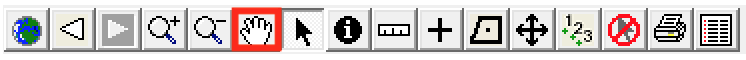
\includegraphics[width=10.36in]{images/toolbar-pan}

The pan tool lets users ``pan and scan'', i.e.~it lets users point,
click, and drag the map in a specific direction. Click on this tool to
recenter the map. The mouse pointer will become a hand - click the map
and move it in any direction.

\hypertarget{select}{%
\subsection{Select}\label{select}}

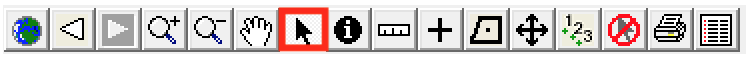
\includegraphics[width=10.36in]{images/toolbar-select}

The select tool allows users to select trees in three ways: point and
click, polygon select, box select.

\hypertarget{identify}{%
\subsection{Identify}\label{identify}}

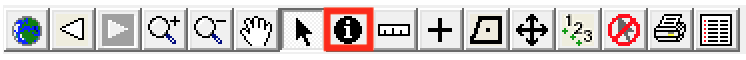
\includegraphics[width=10.36in]{images/toolbar-identify}

The Identify tool allows users to inspect the details of a tree. One the
tool is selected, clicking a tree will open the \emph{Tree Detail}
window which displays tree characterists and work history.

\hypertarget{measure}{%
\subsection{Measure}\label{measure}}

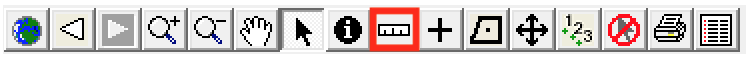
\includegraphics[width=10.36in]{images/toolbar-measure}

The measure tool allows users to measure distances.

\hypertarget{add-tree}{%
\subsection{Add Tree}\label{add-tree}}

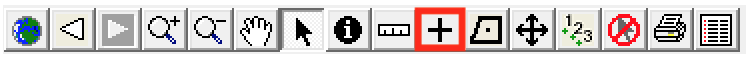
\includegraphics[width=10.36in]{images/toolbar-add-tree}

Click this tool then click on the map to add a new tree. By default, the
characteristics in the Detail form are taken from the nearest tree. This
simplifies the data input as typically just a few things need to be
changed. Remember to click on the Save button to save these
characteristics.

\hypertarget{add-polygon}{%
\subsection{Add Polygon}\label{add-polygon}}

Click this tool then click on the map to add a new polygon. If trees are
the currently selected group to the left of the map or if trees are the
only option, this polygon becomes a Tree Stand.

\hypertarget{move-point}{%
\subsection{Move Point}\label{move-point}}

Click this tool when there are one or more trees selected to move the
selected trees. Click on the map, hold the mouse button down, then move
the mouse and release the mouse button. All selected trees are moved
that distance. If there are selected trees outside the map view,
ArborPro asks whether you wish to move them too.

\hypertarget{site-numbering}{%
\subsection{Site Numbering}\label{site-numbering}}

\hypertarget{clear-selection}{%
\subsection{Clear Selection}\label{clear-selection}}

Clear the selected (in red) and highlighted (in yellow) trees. This also
removes the numbered dots on tree lists.

\hypertarget{print-map}{%
\subsection{Print Map}\label{print-map}}

Click on this tool to print the map the way it currently looks in
ArborPro. A neat line, logo, and text are included. Text on the bottom
of the print page is specified beforehand using the File \textgreater{}
Page Setup menu.

\hypertarget{list-editor}{%
\subsection{List Editor}\label{list-editor}}

Opens the List Edtitor to create a new list, delete the selected trees
from a list, or add the selected trees to an existing list.

\hypertarget{interface}{%
\chapter{Interface}\label{interface}}

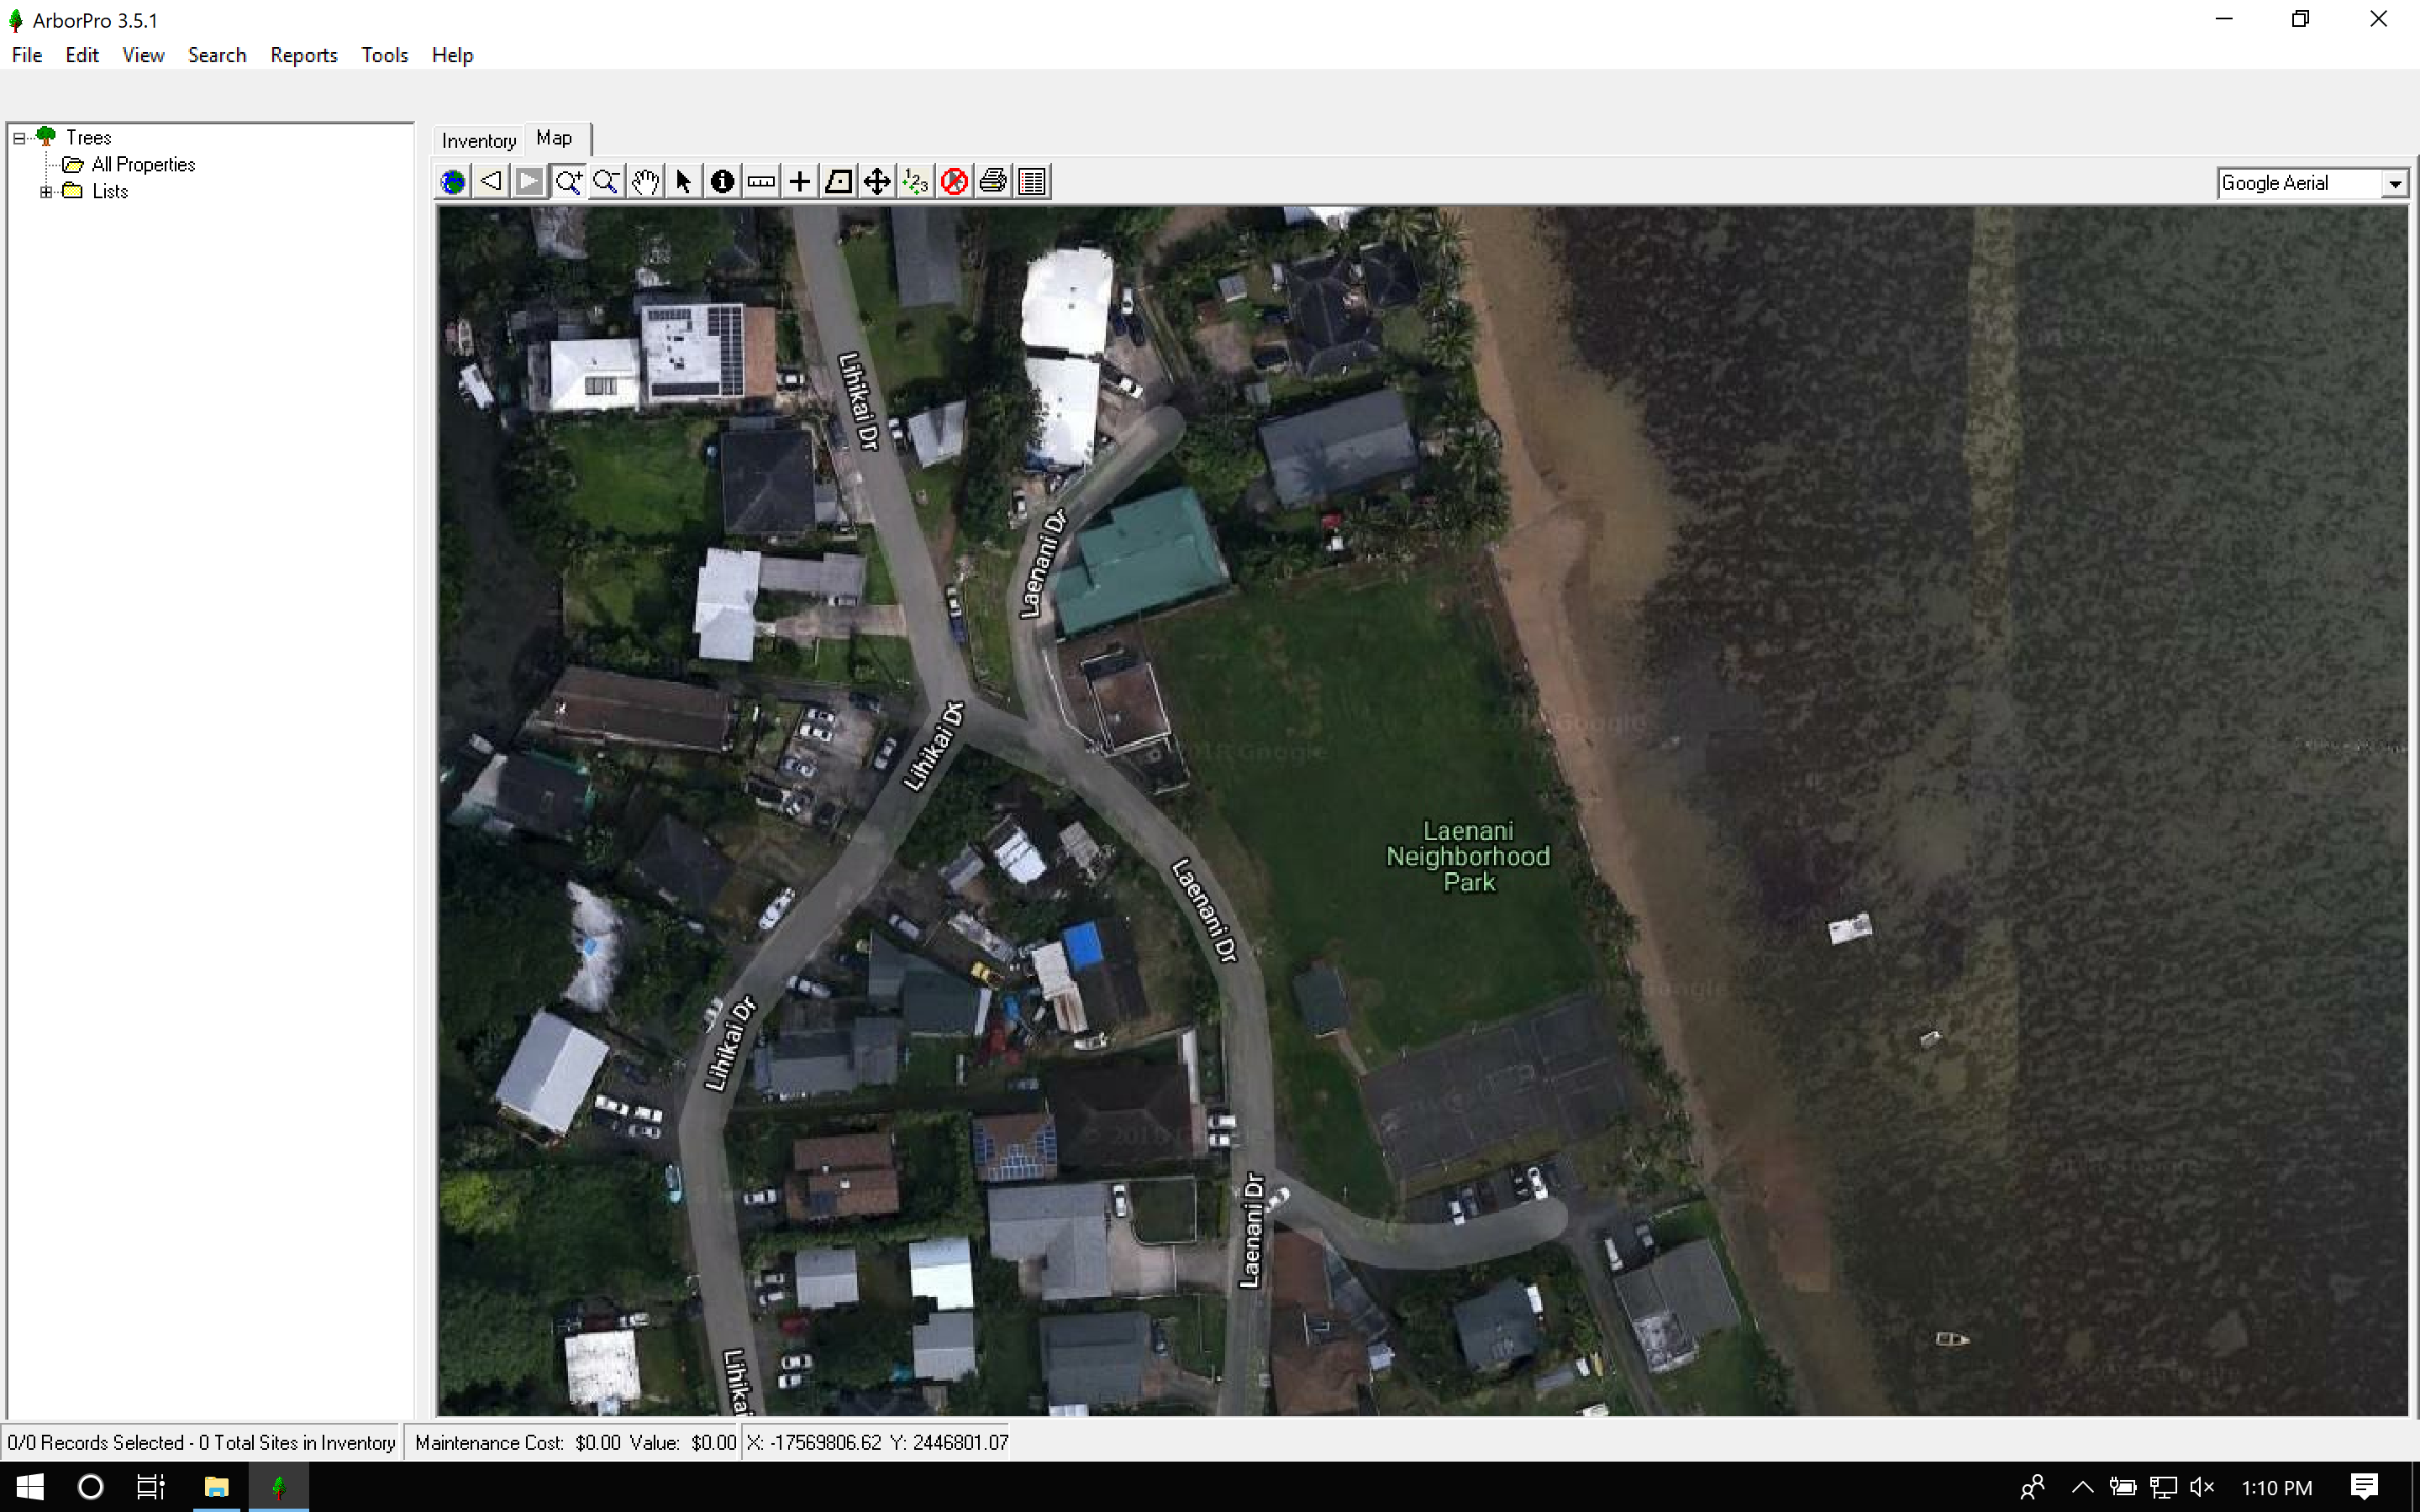
\includegraphics[width=40in]{images/interface}

\hypertarget{the-four-main-components}{%
\section{The Four Main Components}\label{the-four-main-components}}

The ArborPro interface can be broken down into four sections:

\begin{enumerate}
\def\labelenumi{\arabic{enumi}.}
\tightlist
\item
  The map tab
\item
  The inventory tab
\item
  The left panel
\item
  The tool bar
\end{enumerate}

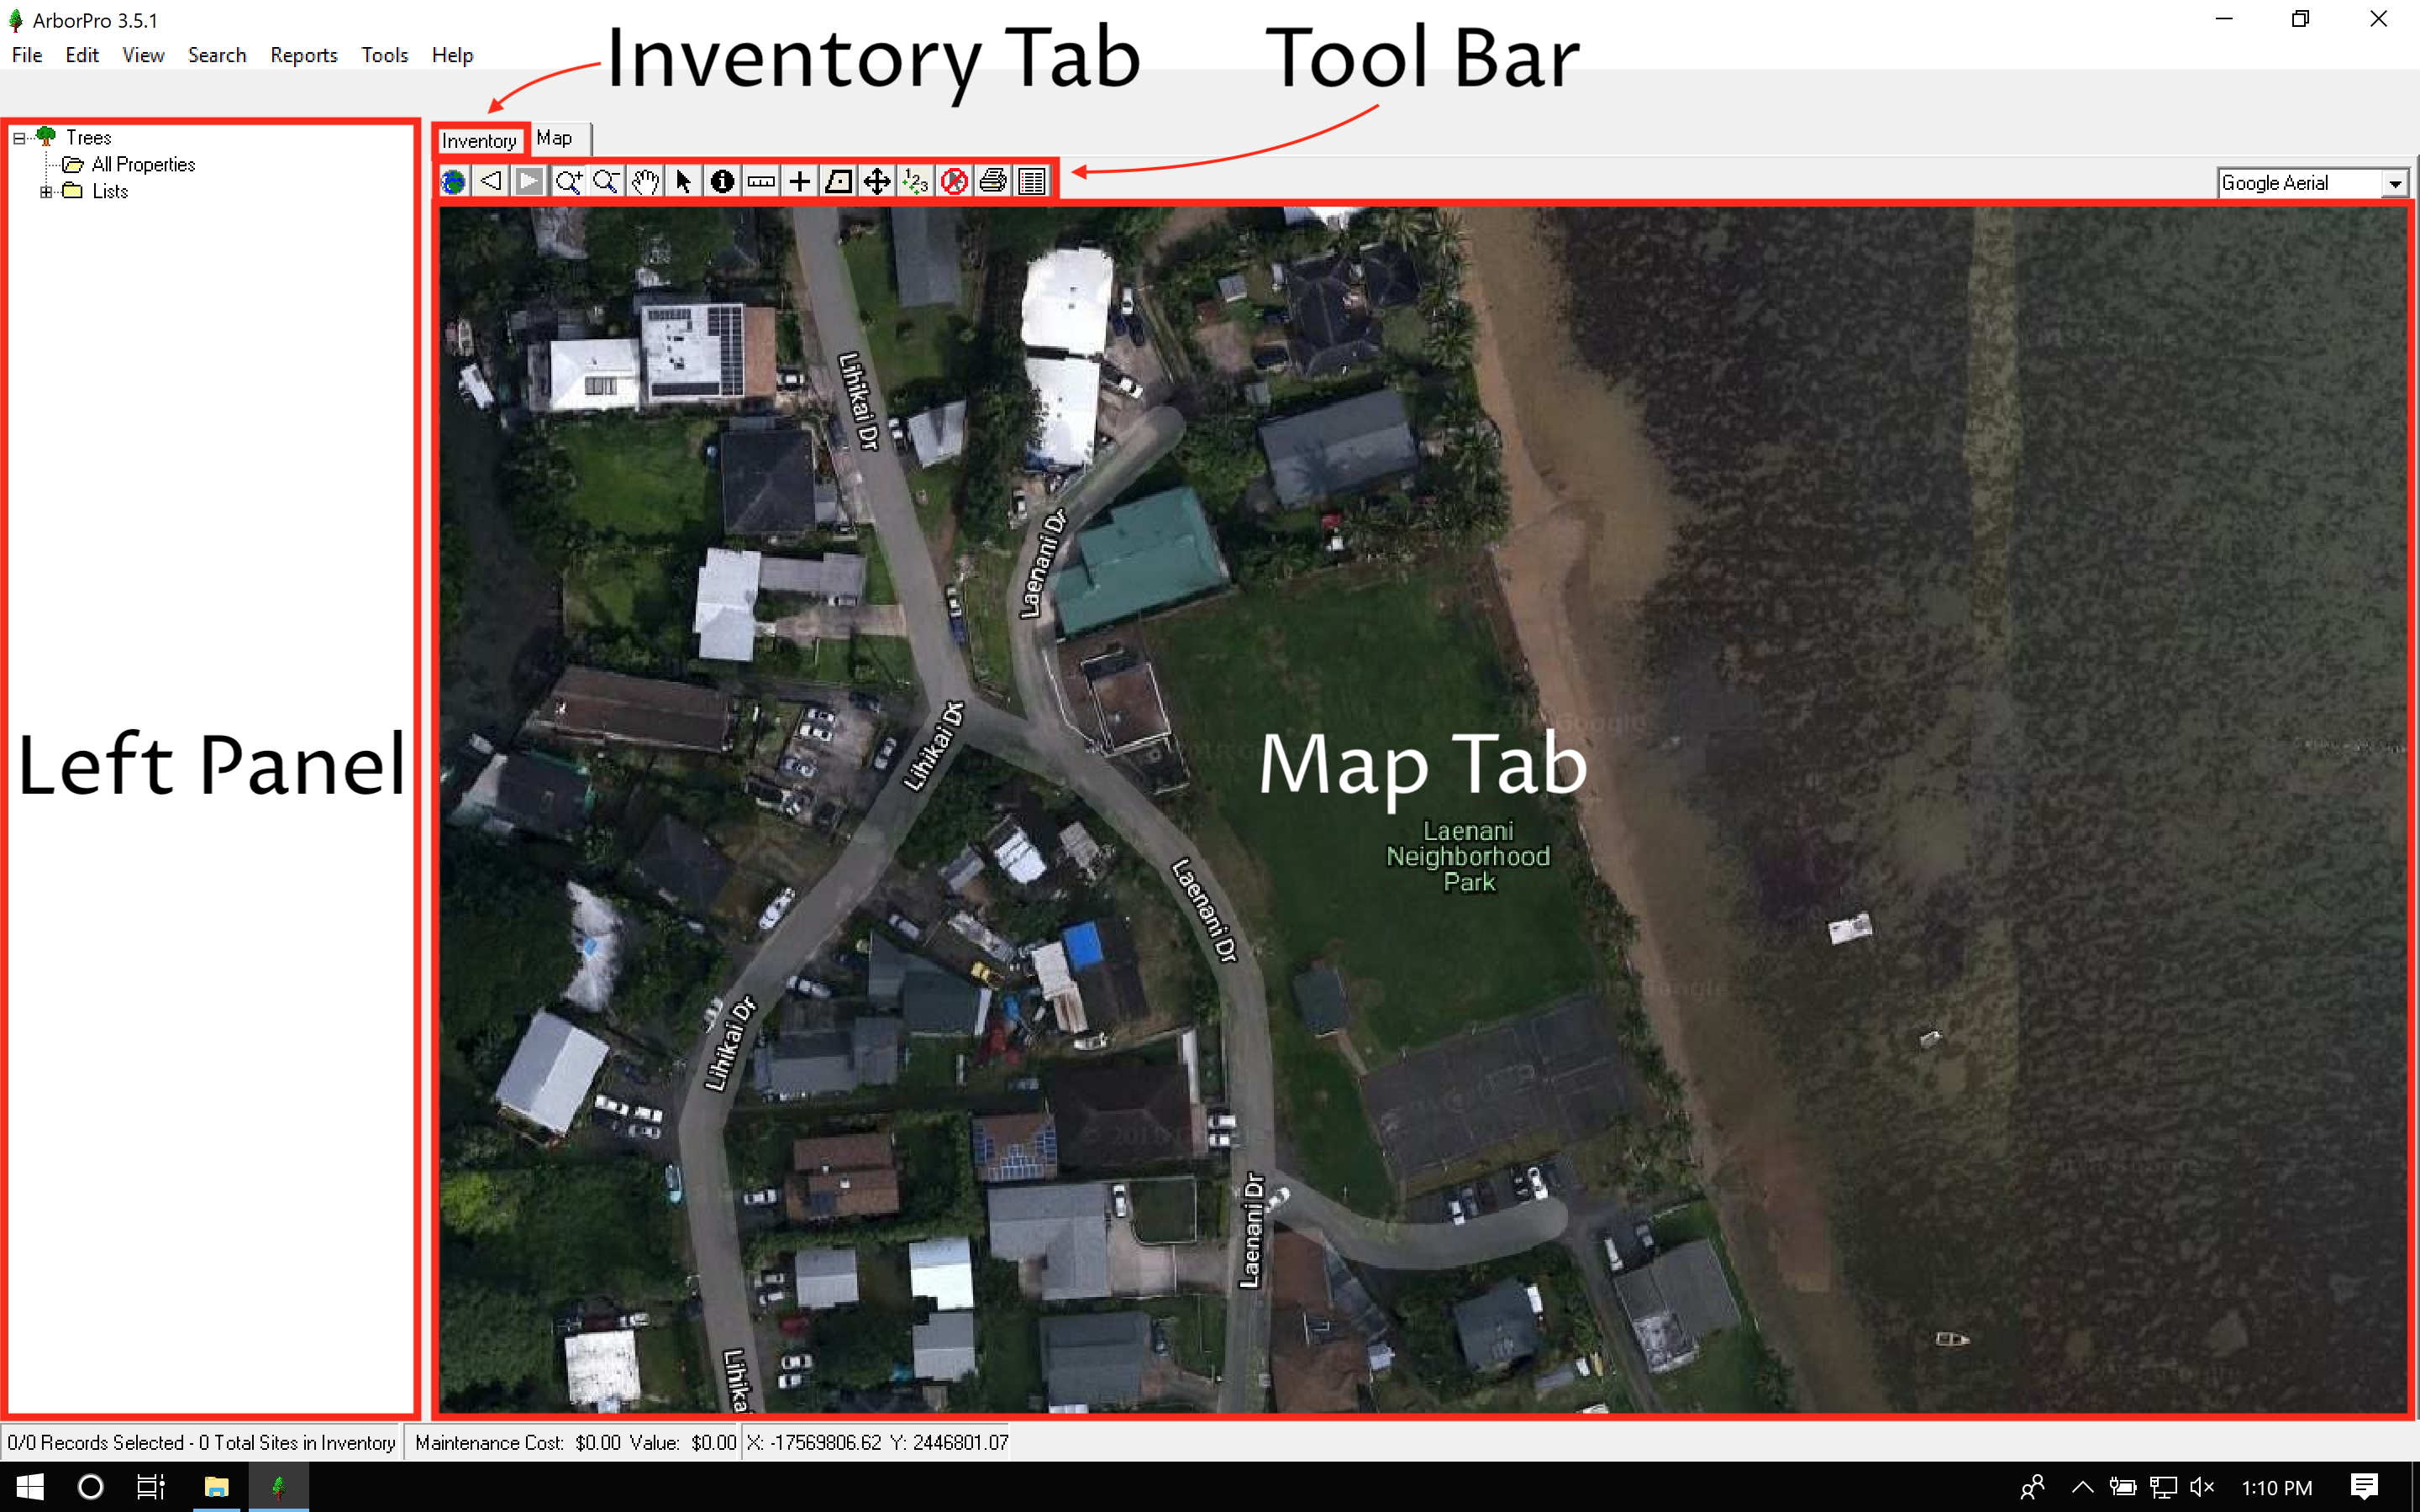
\includegraphics[width=40in]{images/interface-labelled}

In short, the map tab displays the map, the inventory tab displays the
data as a spreadsheet, the left panel organizes properties and lists,
and the tool bar organizes all available tools. We will go over all four
components in more detail below.

\hypertarget{the-map-tab}{%
\subsection{The Map Tab}\label{the-map-tab}}

\hypertarget{the-inventory-tab}{%
\subsection{The Inventory Tab}\label{the-inventory-tab}}

Selecting the inventory tab will display the data as a spreadsheet with
columns and rows. For users comfortable with excel, the inventory tab
should look pretty familiar\footnote{Note that no data is displayed in
  the inventory view because the screenshot was taken from a fresh
  ArborPro install with an empty database.}.

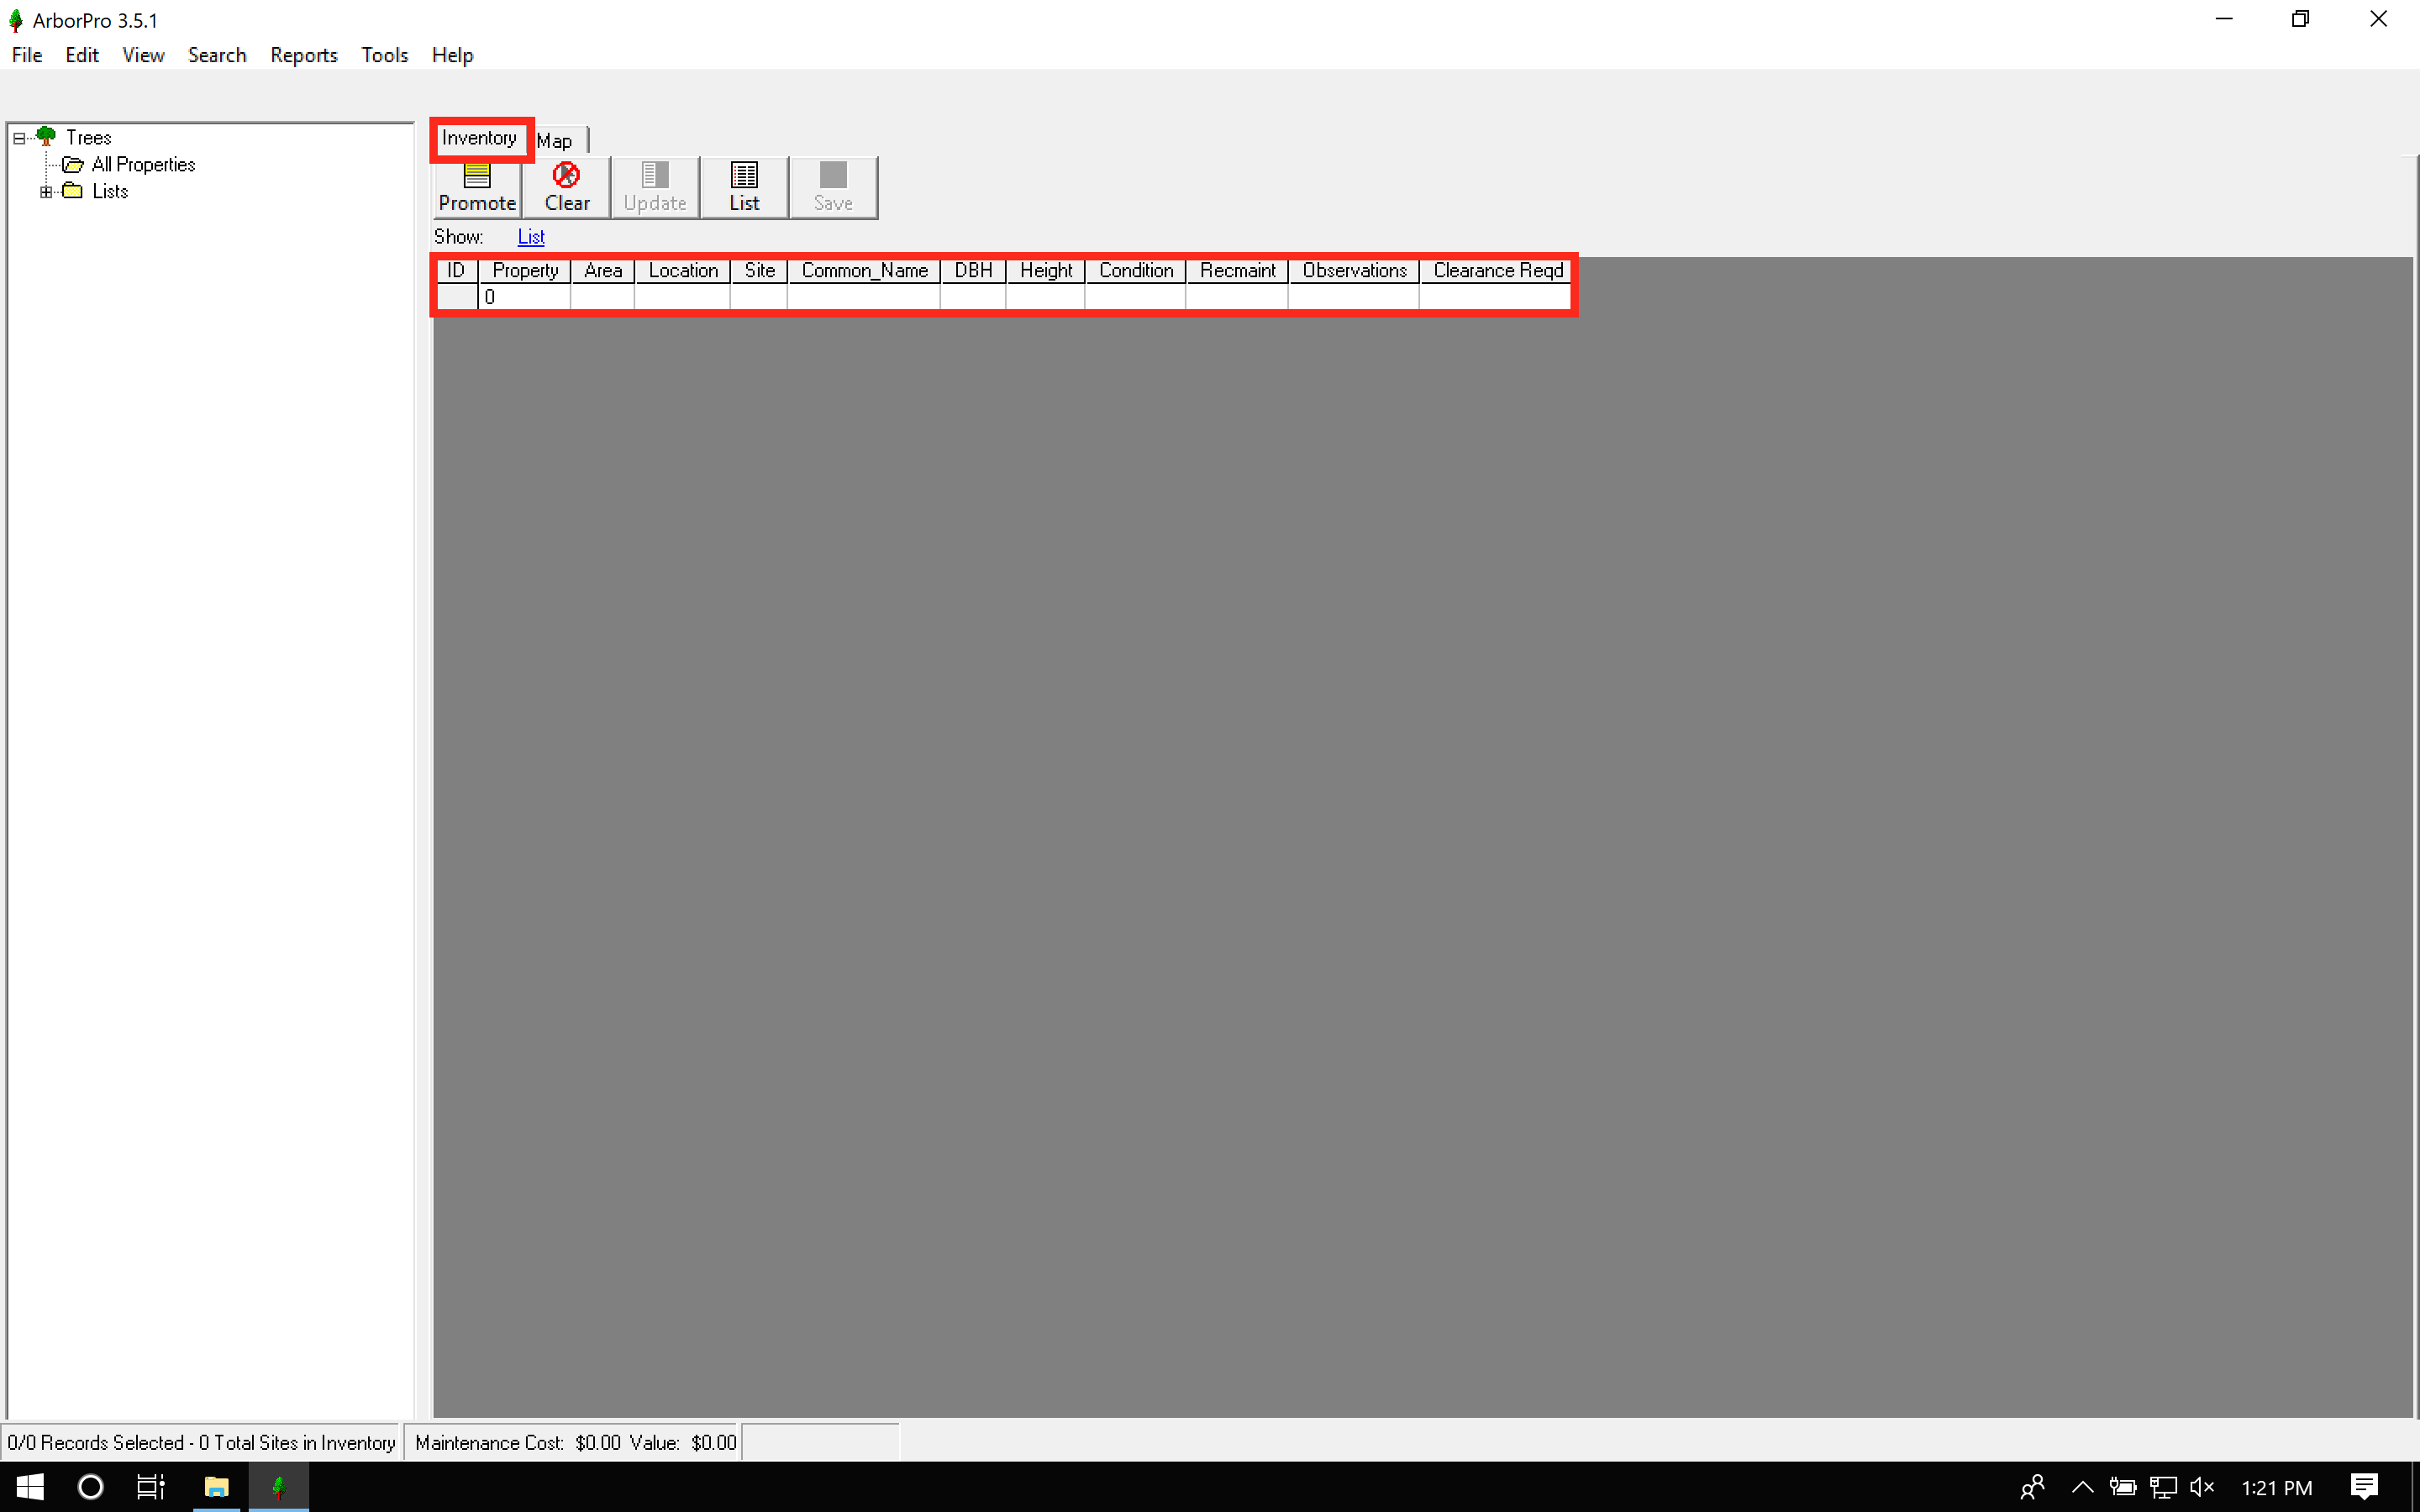
\includegraphics[width=40in]{images/inventory-tab}

\hypertarget{the-left-panel}{%
\subsection{The Left Panel}\label{the-left-panel}}

\hypertarget{the-tool-bar}{%
\subsection{The Tool Bar}\label{the-tool-bar}}

\hypertarget{applications}{%
\chapter{Applications}\label{applications}}

Some significant applications are demonstrated in this chapter.

\hypertarget{identify-hazardous-trees}{%
\section{Identify Hazardous Trees}\label{identify-hazardous-trees}}

\hypertarget{build-a-custom-report}{%
\section{Build a Custom Report}\label{build-a-custom-report}}

\hypertarget{personalize-your-map}{%
\section{Personalize Your Map}\label{personalize-your-map}}

\hypertarget{export-data}{%
\section{Export Data}\label{export-data}}

\hypertarget{exportimport-maintenace-data}{%
\section{Export/Import Maintenace
Data}\label{exportimport-maintenace-data}}

\hypertarget{mass-update}{%
\section{Mass Update}\label{mass-update}}

\hypertarget{summary}{%
\chapter{Final Words}\label{summary}}

We have finished a nice book.

\bibliography{book.bib,packages.bib}


\end{document}
